\chapter{骨质疏松与骨质软化}

骨质疏松为单位体积的骨组织量低于正常,骨组织虽能充分钙化,但骨量不足,致使骨皮质和骨小梁变薄变少。骨质软化系指骨结构钙化不足,在组织学上骨基质正常,而缺少钙、磷等矿物质。

骨的生成可分为两个过程:①由于成骨细胞的活动而构成骨基质,如骨基质生成障碍,则可引起骨质疏松;②骨基质经过羟磷灰石(hydroxyapatite)的沉着而矿质化,如不发生沉钙作用与矿质化,则骨成熟障碍而引起骨质软化或佝偻病。

骨中的无机盐主要是钙和磷的化合物,并与体液中的钙、磷处于动态平衡。成骨细胞中含有丰富的碱性磷酸酶,有促进钙磷沉积的作用。在没有肝脏病和阻塞性黄疸时,血清碱性磷酸酶是成骨细胞活动的一个指标,同时也是骨基质形成的一个指标。体液中所含的钙和磷虽少,但意义甚大,一方面反映骨质代谢的情况,另一方面反映这两种物质在肠道吸收以及由肾与肠道排泌的情况。正常情况下借体液传输的作用,骨质的钙、磷含量与摄入量维持平衡。这种平衡之所以得以维持,除与食物进量有关以外,还需依靠骨组织和消化道、肾脏等器官的功能,以及有赖于维生素、内分泌和中枢神经系统的调节。

目前,临床上诊断骨质疏松或脱钙已不全依靠骨骼的X线检查,X线所见的骨质疏松不一定就是真正的骨质疏松,往往仅提示由于骨钙量不足而呈现的骨质缺乏。骨质缺乏可有下列三种可能性:①真正的骨质疏松;②骨质软化;③骨质纤维化(纤维性骨炎)。此三种骨质缺乏病的鉴别参见表\ref{tab39-1}。

骨质疏松的诊断过去主要依靠X线摄片检查。骨密度测量能反映全身或局部矿化骨的含量,其优点还在于其非创伤性。骨密度测量可为临床提供一项早期诊断骨量减少和骨质疏松、预示骨折危险性的敏感和有效的检查方法,特别宜用于老年患者。由于常规X线摄片不能发现少于30\%~50\%的骨质丢失,应用双光子密度吸收法(DPA)、双能X线吸收法(DEXA)或定量超声骨质测量等技术测定骨密度作定量判断较为适当。

定量CT(QCT)在评价多种形式的骨质疏松方面,具有高度准确性的优点,因而有广泛应用的潜力。

骨活检是诊断骨病的金标准,但为创伤性检查。QCT和放射性核素\textsuperscript{99m}
Tc扫描提供非创伤性有价值的检查方法。关于普遍性(或局限性)骨质缺乏的疾病,将于下文表述(表\ref{tab39-2})。

\begin{table}[htbp]
\centering
\caption{三种骨质缺乏的鉴别}
\label{tab39-1}
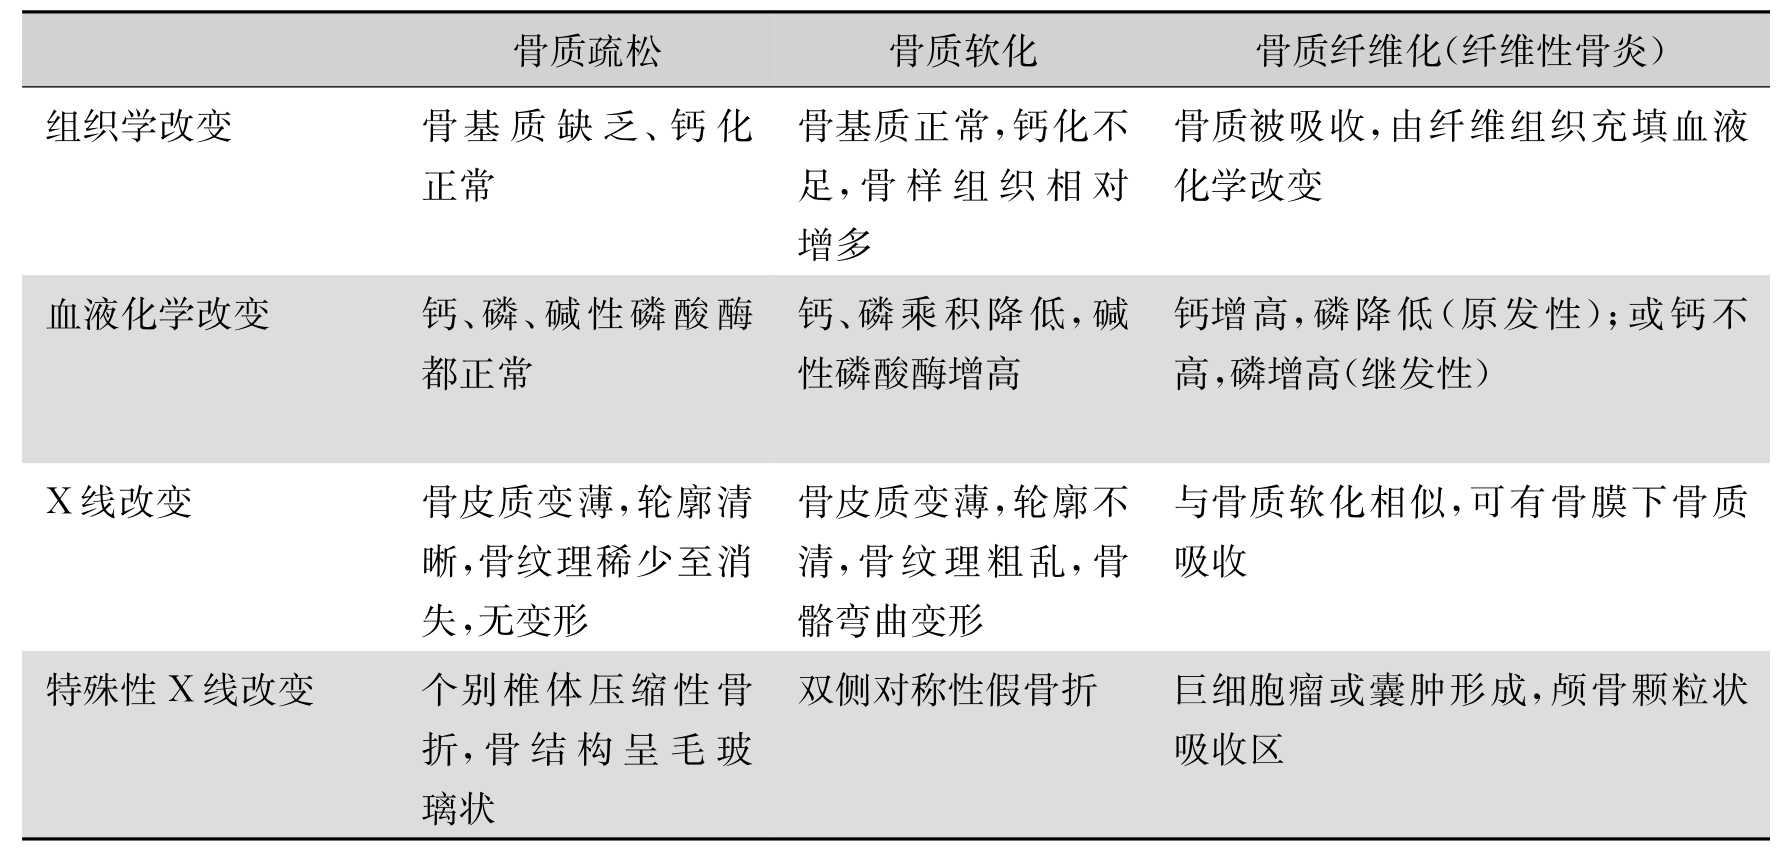
\includegraphics[width=5.96875in,height=2.83333in]{./images/Image00244.jpg}
\end{table}

\begin{table}[htbp]
\centering
\caption{普遍性(或局限性)骨质缺乏的疾病}
\label{tab39-2}
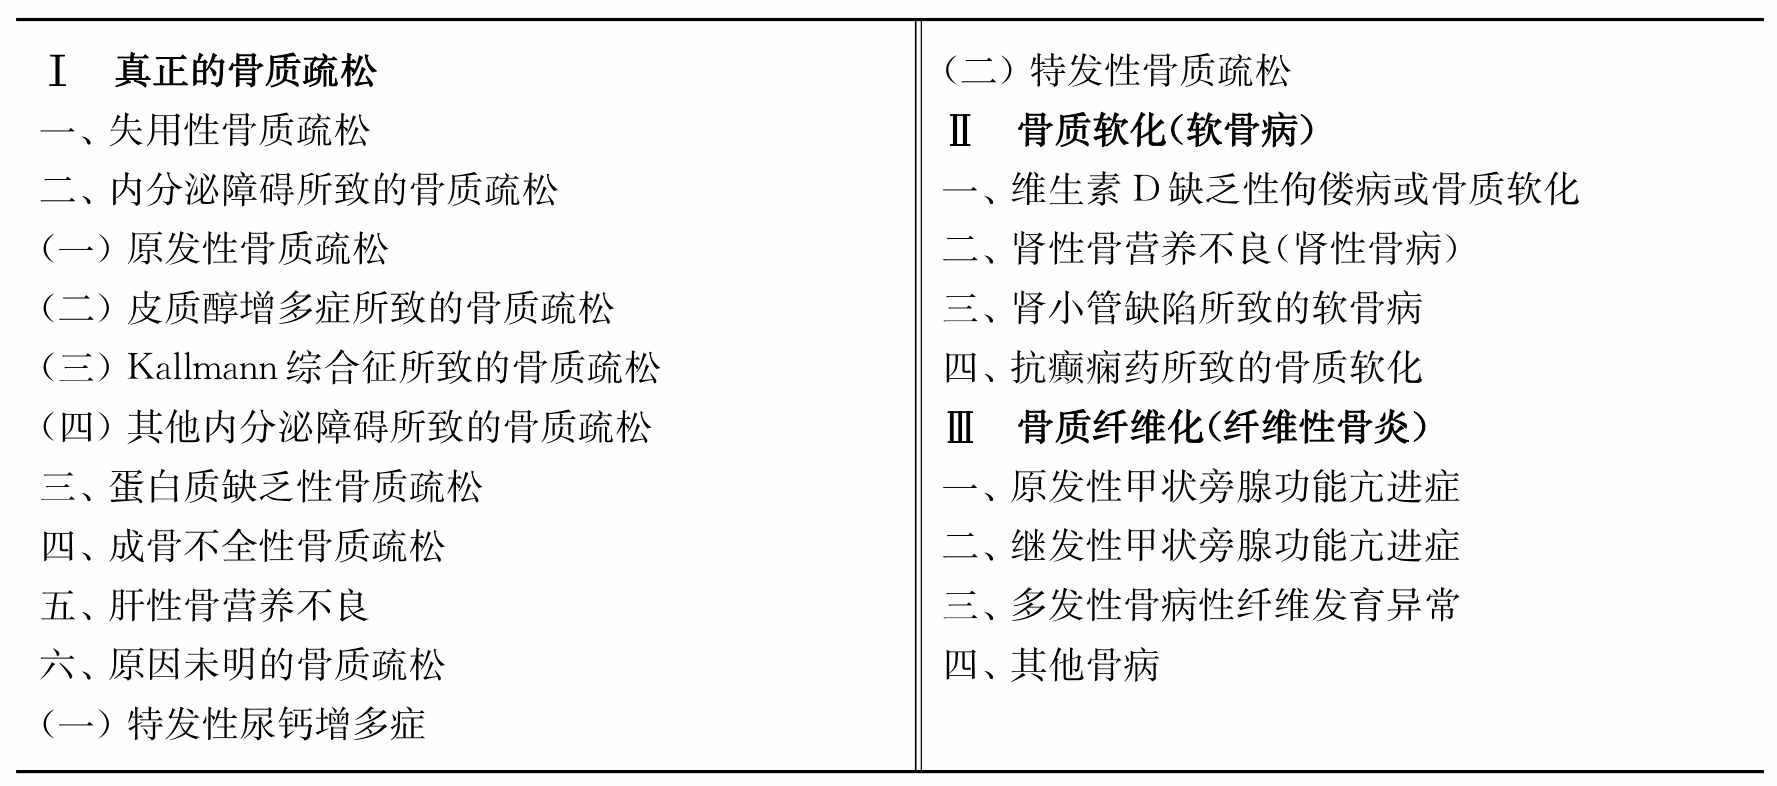
\includegraphics[width=5.91667in,height=2.61458in]{./images/Image00245.jpg}
\end{table}

\protect\hypertarget{text00307.html}{}{}

\section{129 真正的骨质疏松}

真正的骨质疏松是骨生成障碍的结果。乃由于成骨细胞活动力降低所致,患者常有临床三联症:骨痛、骨弯曲和易于骨折。

骨质疏松时血清钙、无机磷与碱性磷酸酶大致正常,故与骨质软化有所不同。尿钙排泄有时增多,在此情况下可引起尿路结石形成。真正的骨质疏松有如下几种:

\subsection{一、失用性骨质疏松}

失用性骨萎缩所致的骨质疏松可为普遍性或局限性。这种情况可见于长期全身或局部活动过少。肢体瘫痪、慢性骨关节疾病或因骨折长期固定的肢体,使成骨细胞缺乏必要的刺激。成长中的儿童及活跃的成人,如因某些疾病引起急性瘫痪(例如脊髓灰质炎),当大量的骨形成正在进行但对骨形成的刺激突然中止时,则出现所谓急性失用性骨质疏松。其实验室检查特点是血清钙、磷数值均可增高,碱性磷酸酶正常或下降,与原发性甲状旁腺功能亢进症的鉴别多无困难,后者以血钙升高、血磷降低、碱性磷酸酶明显升高为特征。

\subsection{二、内分泌障碍所致的骨质疏松}

\subsubsection{(一)原发性骨质疏松}

雌激素有刺激成骨细胞功能的作用,故妇女在绝经期后可发生骨质疏松,尤以腰椎明显,受外力压迫可引起压缩性骨折。老年男子也有发生骨质疏松者,因雄激素有促进蛋白质合成的作用,雄激素缺乏时骨基质的蛋白质合成不足,从而出现骨质疏松。实际上,生理性老年性骨质疏松是由于性激素缺乏、消化功能减退(如胃酸减少或缺乏)、蛋白质摄入不足、体力活动过少等一系列综合性因素所致。腰背痛与骨痛是早期症状。

绝经后骨质疏松的诊断往往被忽略。骨质疏松时骨质减少通常无症状,患者通常在骨折发生后才来求诊。绝经后头10年易发生前臂远端的Colles骨折,10年之后才出现椎体压缩性骨折,而髋部骨折多发生于75岁之后。椎体压缩性骨折可自发发生或发生于轻微活动之后,患者可感到背痛,脊柱畸形或驼背,身高降低,严重者可出现其他部位的多发性骨折。骨密度测量目前多采用单(双)光子吸收法、双能X线吸收法或定量计算机断层摄影(QCT)等方法测定骨矿物质密度(BMD),其准确性和精密度大大提高

\subsubsection{(二)皮质醇增多症所致的骨质疏松}

Cushing综合征患者常发生骨质疏松,有时甚至出现自发性骨折。国内60例库欣综合征出现骨质疏松者占71.6\%,4例伴有自发性骨折。颅骨蝶鞍前、后床突骨质疏松较其他部位先出现。患者的骨质疏松主要由于糖皮质激素作用于骨的间质,引起蛋白质合成抑制及分解亢进。血生化学检查血清钙大致在正常范围,血清碱性磷酸酶早期多正常,晚期可稍升高。

长期应用促皮质激素或糖皮质激素治疗时,有报告2\%~10\%发生骨质疏松。

\subsubsection{(三)Kallmann综合征}

主要临床表现为性腺发育不良、嗅觉丧失综合征,骨质疏松亦为突出表现。病因为低促性腺激素所致的性腺功能过低,罹患多为男性。

\subsubsection{(四)其他内分泌障碍所致的骨质疏松}

肢端肥大症、甲状腺功能亢进症、糖尿病等都可引起骨质疏松。通常临床症状为骨痛,少数可出现病理性骨折,主要与内分泌代谢失调有关。

\subsection{三、蛋白质缺乏性骨质疏松}

肝硬化、肾病综合征、血液病、脂肪泻、营养不良等所致的骨质疏松均属此类。病因通常为综合性。蛋白质缺乏或大量丢失、维生素C及D缺乏、胃肠功能障碍、附加感染等均为发病的有关因素。

\subsection{四、成骨不全性骨质疏松}

成骨不全性骨质疏松是遗传性疾病,是由于成骨细胞功能缺陷,不能形成骨基质所致。临床上区分为先天性与迟发性二种。患者有自发性骨折倾向,自幼年至老年常屡次发生自发性骨折,典型病例尚有其他先天性缺陷的征象,如神经性耳聋(因耳硬化所致)或(及)巩膜呈蓝色(因巩膜变薄,能透视血管丰富的脉络膜)。X线摄片检查可见骨质薄而含钙减少,常并发多发性骨折征,有新旧不等的骨痂及弯曲畸形。血清碱性磷酸酶大多增高,而血清钙、磷正常,尿钙与尿磷排泄也正常。

\subsection{五、肝性骨营养不良(肝性骨病)}

有作者用生化分析、单光子扫描技术研究112例各种类型的病毒性肝炎患者,发现多有不同程度的低血钙、高血磷、低骨密度改变。慢性肝炎患者组明显高于急性肝炎患者组。作者认为,病毒所致的肝病存在着普遍的骨营养不良。低钙型膳食以及病毒对肝、肾的损害,可能是肝性骨病的主要原因。

\subsection{六、原因未明的骨质疏松}

\subsubsection{(一)特发性尿钙增多症}

本病非常罕见,特点是尿钙高,有骨质疏松征象及血清碱性磷酸酶增高,与甲状旁腺功能亢进症相似,所不同者是本病血钙正常或偏低,血磷正常或偏高,尿磷低,骨质疏松无纤维性囊性改变。血钙不高而尿钙增高的原因未明。

\subsubsection{(二)特发性骨质疏松}

本病原因未明,故称特发性骨质疏松。有人认为可能由于骨基质形成与成骨细胞活动性存在着先天性缺陷。多见于青年人,不限性别。内分泌腺功能正常。罹患部位以椎骨及盆骨最显著。临床表现与绝经期或老年性骨质疏松相同,但患者并非绝经期或老年人,也未发现任何其他原因。血清钙、磷与碱性磷酸酶均大致正常,但有钙与磷代谢负平衡的表现。

\protect\hypertarget{text00308.html}{}{}

\section{130 骨质软化(软骨病)}

骨质软化是成年人的佝偻病,原因是由于钙吸收不足(吸收性骨质软化)或钙排出增多(排泄性骨质软化)。女性罹患多于男性。

患者最早的症状是腰腿疼痛,继而骨骼出现压痛,行动困难。早期症状应与风湿性关节炎相区别。疼痛自腰腿蔓延至胸胁及上肢;性质多种多样,但以酸痛与刺痛居多;程度轻重不等,重者难以忍受,夜间不能自动翻身。妊娠期患者的疼痛往往于妊娠4~5个月后加剧。长期过程易引起脊椎、胸廓、骨盆及下肢骨骼变形,或发生病理性骨折。

血生化学检查血清钙、磷值下降或正常,碱性磷酸酶大多增高。

根据发病原因,骨质软化可分为:

\subsection{一、维生素D缺乏性佝偻病或骨质软化}

本病又名吸收性骨质软化,在华南地区十分罕见。华南地区属亚热带气候,阳光终年照射,居民也有穿短衣的习惯,故甚少患维生素D缺乏。国内报告病例主要见于华北、东北、内蒙古等地区。气候条件与生活习惯,尤以饮食习惯为主要致病因素。发病多在冬季,症状也以冬季严重。绝大多数发生于生育较多的妇女。妊娠为重要的促发因素。

此外,偶尔因长期腹泻(如脂肪泻、慢性胰腺炎)或阻塞性黄疸,也可引起维生素D吸收障碍并导致骨质软化。

家族性骨软化症是一种遗传性疾病,近年国内有二组家族性骨软化症的报道,其患病成员均有低血钙、低血磷与血清碱性磷酸酶活性增高,X线片示有骨质疏松或骨软化的表现。一组患者似为常染色体显性遗传,用大剂量维生素D及钙剂治疗有效;另一组的遗传类型不同于前者,用钙剂及小剂量维生素D治疗即有明显的效应。

\subsection{二、肾性骨营养不良(肾性骨病)}

肾性骨营养不良是慢性肾衰竭患者一系列内分泌代谢异常所致的骨综合征。常见症状为骨痛,严重者可致病理性骨折。病理检查所见为骨软化、纤维性骨炎等。骨活检是最佳的诊断手段,能准确了解骨和骨前质的量、质和结构,骨细胞的数目、功能以及骨的运转和重建状况,对骨病的诊断、鉴别诊断和治疗选择是不可缺少的手段。

广义的肾性骨病是指一切和肾脏问题有关的骨病,如肾小管酸中毒时发生的骨质软化,透析膜组织不相容发生的淀粉样骨病等。而狭义的、通常简称的肾性骨病是指伴发于慢性肾衰竭的代谢性骨病。重症者因四肢长骨及脊柱骨脱钙而致身高缩短,称退缩人综合征。

近年学者们对下列几种肾性骨病曾分别加以论述:

\subsubsection{(一)高转化性骨病}

本病的组织学改变多表现为纤维性骨炎和混合性骨病。慢性肾功能不全患者几乎100\%均有甲状旁腺激素增高。有作者报道甲状旁腺激素>45μg/L,诊断高转化骨病的特异性达100\%。

\subsubsection{(二)低转化骨病}

目前认为低转化骨病的骨软化与骨铝过多密切相关。本病的特点是:①发病多为老年(>50岁)、糖尿病和腹透患者;②血清生化指标为血钙浓度高、甲状旁腺激素水平低下;③从发现肾功能不全到开始透析的时间长;④血管钙化的发生率高;⑤组织学上表现为以骨矿化缺陷为主。

\subsubsection{(三)混合性骨病}

以上两种因素并存所致的混合性骨病。

\subsection{三、肾小管缺陷所致的软骨病}

近年有作者报道成人骨软化症13例,平均年龄34.1岁。其中抗维生素D性佝偻病5例、肾小管酸中毒合并骨软化症6例、范科尼综合征2例。据此组材料,可见肾小管缺陷是成人骨软化症的常见原因之一。

抗维生素D性佝偻病是一种性联显性遗传性疾病,因肾近曲小管重吸收磷障碍及肠吸收钙不良所致。临床表现与维生素D缺乏性佝偻病相似,但对维生素D治疗无效。患者血钙正常,血磷低,血钙、磷乘积低于20,尿磷增加。当遇有佝偻病而无维生素D缺乏史,又无氮质血症或其他肾小管功能缺陷疾病时应考虑本病,如有家族病史或家族成员中有低磷血症时更支持本病。本病临床上极罕见。

肾性骨营养不良、维生素D缺乏性佝偻病或骨质软化、原发性甲状旁腺功能亢进症的实验室检查鉴别见表\ref{tab39-3}。\footnote{正常每100ml血浆中钙和磷含量的乘积为36~40;↑:增加;↓:减少}

\begin{table}[htbp]
\centering
\caption{肾性骨营养不良、维生素D缺乏性佝偻病或骨质软化、原发性甲状旁腺功能亢进症的实验室检查鉴别}
\label{tab39-3}
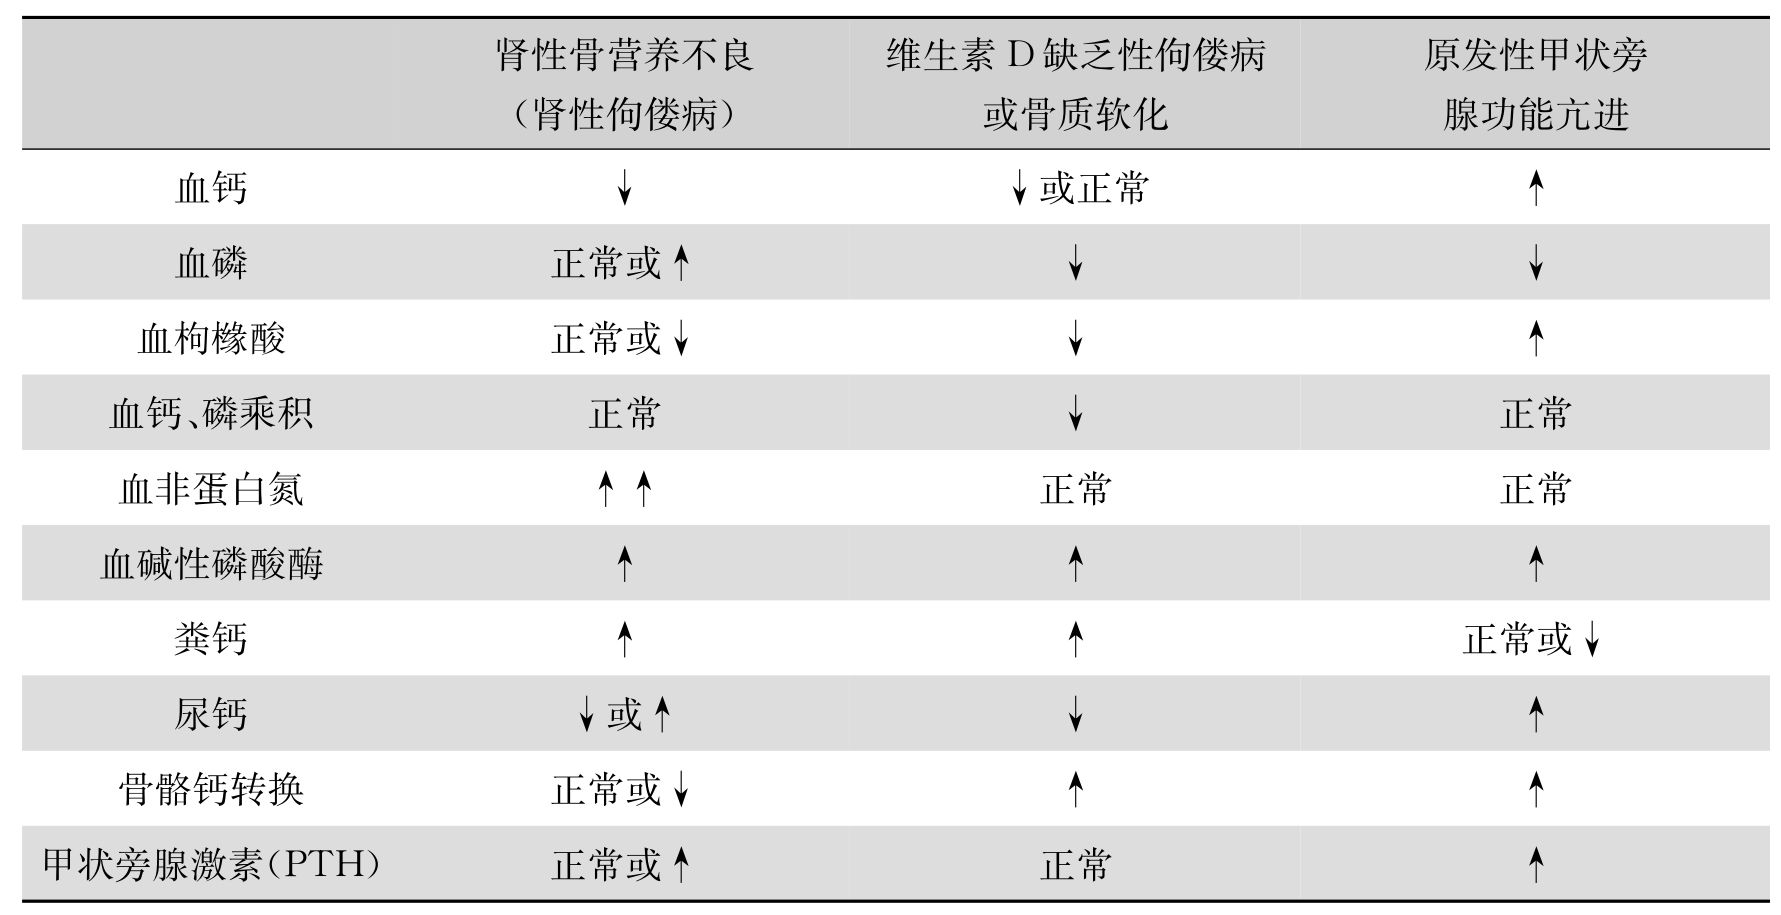
\includegraphics[width=5.92708in,height=3.04167in]{./images/Image00246.jpg}
\end{table}

\subsection{四、抗癫痫药所致的骨质软化}

1968年Kruse曾首次报告在抗癫痫药治疗的病儿中,15\%出现佝偻病的骨X线改变,伴血钙与血磷降低,血清碱性磷酸酶升高。患者无营养缺乏,光照充足,肾功能正常,无酸中毒,确诊为抗癫痫药治疗所致。发病机制尚未充分明了。此病国内、外陆续有报告。

\protect\hypertarget{text00309.html}{}{}

\section{131 骨质纤维化(纤维性骨炎)}

\subsection{一、原发性甲状旁腺功能亢进症}

原发性甲状旁腺功能亢进症通常由单个、有时由多个甲状旁腺腺瘤所引起,少数由于腺体增生或癌所致。女性患者3倍于男性。症状的发生乃由于甲状旁腺激素分泌增加,此种激素的作用是:①作用于肾脏,抑制尿中磷酸盐的重吸收,致磷酸盐排出增多,并引起多尿及血磷降低;②直接作用于骨组织,使之脱钙,血清钙升高,尿钙也随之增加。

临床症状较少特征性,可归纳为下述三组:①高钙血症症状:表现为疲乏无力、体重减轻、食欲缺乏、便秘,有时呕吐、上腹痛、心动过速,精神症状如淡漠、抑郁等。当血钙急剧升高超过15mg/100ml时,可诱发急性甲状旁腺功能亢进症(甲状旁腺危象),主要表现为呕吐、多尿、发热、高度脱水与精神失常,此时多伴有血磷升高;②泌尿系症状:烦渴、多尿,病程较长者可出现肾结石、血尿等征象,易并发肾盂肾炎或肾功能不全;③骨病变:表现为腰背及肢体的风湿样痛,甚至发生自发性脊椎、长骨与肋骨骨折,末指(趾)节骨缩短。

本病临床上可分为五个类型:①以骨骼病变为主;②以泌尿系病变为主;③兼有骨骼和泌尿系病变;④兼有溃疡病和泌尿系病变;⑤无明显症状,仅由于其他原因做血钙测定而发现。国外报告以泌尿系病变为主者多见,而国内以骨骼病变较泌尿系病变多见,可能与饮食习惯不同有关。

过去认为原发性甲状旁腺功能亢进症是一种罕见的疾病,可能是由于许多病例被漏诊。从国内的病例来看,患病至确诊时间平均为2~5年,个别延误可达8年之久。故对有多发性骨折或(及)骨畸形、复发性泌尿道结石、溃疡病伴有血尿、复发性胰腺炎等患者应警惕本病的可能性,并进一步作有关的实验室检查证实或除外本病。

实验室检查:高钙血症与低磷血症是本病的典型表现,但非经常存在。如测定数值正常而临床上怀疑本病,需多次复验。碱性磷酸酶升高,其出现先于骨骼X线改变,少数病例达正常值10倍之多。许多早期具有健全骨骼的病例,碱性磷酸酶数值也可正常。血清甲状旁腺激素(PTH)水平增高。

部分患者心电图显示ST段下降,T波倒置,QT间期缩短,提示高钙血症。

尿改变:如无肾功能不全,大多数病例有尿钙、尿磷排出增加。尿钙增加有时表现为排出尿砂。尿钙增多可用尿钙定性试验(sulkowitch法)证明。尿钙定性试液含草酸、草酸铵各2.5g,冰醋酸5g,蒸馏水加到150ml。取试管载等量尿液与试液混合,如2~3分钟后不出现浑浊或仅有轻度浑浊,提示尿钙排量不多;如呈乳样浑浊,则提示尿钙增多。

本病晚期可出现血磷升高、高血压,此时通常也有非蛋白氮升高,提示肾功能不全。X线摄片可出现钙化肾的征象。

X线摄片检查:约1/3的病例可确定单纯的骨质疏松;约1/3呈弥漫性囊性纤维性骨炎的改变,为本病的特征性表现,并可发生骨畸形与骨折,少数病例出现巨细胞瘤样改变;其余1/3的病例并无骨质的X线改变。

原发性甲状旁腺功能亢进症的诊断:

\subsubsection{1.定性诊断}

\paragraph{(1)血钙及血磷测定:}

如血钙>11mg\%、血磷<3.0m\%,则对本病有诊断意义。一般认为血钙在10.5mg\%以下为正常,在10.6mg\%以上为可疑,在11.2mg\%以上就被认为是手术探查的对象。但有些甲状旁腺功能亢进症的血钙可正常。在估计血钙时,需参考血清蛋白量是否正常(如血清总蛋白测定低于6.5g\%时,每低1g需在血钙测定数值上增加1mg),有无维生素D缺乏症和有无肾功能不全的存在。

\paragraph{(2)尿钙测定:}

如无肾功能不全,可在低钙饮食3天后进行24小时尿钙定量测定。正常尿钙24小时排量为12.5mg±50mg,如24小时尿钙含量超过250mg,则有诊断意义。约1/3的病例尿钙定量测定可正常,因此尿钙定量的诊断意义不及血钙。

\paragraph{(3)血清甲状旁腺激素(PTH)测定:}

PTH水平增高与原发性甲状旁腺功能亢进症的严重程度、肿瘤大小及血钙升高的程度有关。PTH水平增高伴高血钙有诊断意义。

\paragraph{(4)应用肾上腺皮质激素鉴别高钙血症:}

高钙血症也可见于多发性骨髓瘤、结节病、维生素D过多症、急性失用性骨质疏松、慢性肾上腺皮质功能减退症、甲状腺功能亢进症、恶性肿瘤或兼有骨转移者。连续7天每天口服氢化可的松100mg或泼尼松20mg,服药前及服药期第3、5、7天测定血钙值,其他高钙血症患者服激素后可见血钙下降,而原发性甲状旁腺功能亢进症不受影响,但也有个别例外。

\paragraph{(5)忌磷试验:}

给予患者低磷饮食(例如每天进食2000kcal热量里含有磷430mg、钙700mg),持续3~6天。在低磷饮食前一天及第3、6天,空腹抽血测定血钙及磷,并收集24小时尿液测定尿磷。本试验在甲状旁腺功能亢进症可见血钙升高、血磷下降而尿磷排量仍高,对诊断原来血钙、血磷接近正常的本病患者有很大帮助。

\paragraph{(6)肾小管磷重吸收率(TPR):}

对肾功能良好的原发性甲状旁腺功能亢进症是比较可靠的诊断方法。在肾功能不全、肾小管疾病、结节病或骨质软化、多发性骨髓瘤等疾病可有假阳性结果。详细方法参考生化检验书籍。正常人肾小管磷重吸收率约界于84\%~96\%,原发性甲状旁腺功能亢进症约界于76\%~83\%。

\subsubsection{2.定位诊断}

国内应用核素显像诊断原发性甲状旁腺功能亢进,方法简便、准确。

\subsection{二、继发性甲状旁腺功能亢进症}

本病常由肾功能不全所引起,故这种状态也称肾性骨营养不良。本病的临床症状与原发性甲状旁腺功能亢进症相似,但骨骼改变罕有如原发性甲状旁腺功能亢进症显著,患者有慢性肾脏疾病与高磷血症。甲状旁腺由于血磷升高而继发增生、肥大,引起功能亢进,血清PTH水平可增高,此时与晚期原发性甲状旁腺功能亢进症并发肾功能不全的鉴别有一定困难。前者有较长期的肾病史,血钙不高,骨骼损害多不显著(仅约1/3的病例有典型的纤维性骨炎),但常有关节周围及皮下钙化现象,有双侧对称性假骨折,碱性磷酸酶仅轻度升高,肾小球磷的廓清率常降低(正常值为10ml/min,原发性甲状旁腺功能亢进症常升高),磷廓清率与肾小管磷重吸收率的比值也降低。

\subsection{三、多发性骨病性纤维发育异常}

多发性骨病性纤维发育异常(polyostotic fibrous
dysplasia)是一种较少见的骨病,国内有多例报告。本病兼有性早熟现象者称Albright综合征。此综合征几乎仅见于女性,病因未明,可为遗传性,其三联症是:骨病变(脱钙、纤维性变性、骨弯曲与骨折)、性早熟(可能病变在第三脑室壁所致)与皮肤色素异常(大色素斑形成)。骨病变为局限性而非普遍性,有好发于同一侧骨骼的倾向,患骨的髓腔及骨皮质为具有不同程度骨化的纤维组织所代替,尚出现局部密度增高(毛玻璃征)、密度减低(囊变征)及患骨膨大弯曲畸形等。血钙及其他生化检查均正常。于5~15岁之间首次出现明显症状,青春期后病程停止进行。此综合征国内有多例报告。如无色素异常与性早熟,称为多发性骨病性纤维发育异常,在成年期间可发生骨折。多发性骨病性型的X线像甚为特别,对本病的诊断有决定性意义。单发性骨病性型常需依赖活组织检查方能确诊。

本病的组织学特征与纤维性骨炎很相似,两者的X线征也相似,但两者的不同点也很多。本病是一种局限性疾病,虽然损害可为广泛性,但其他部位常有不受累及的正常骨骼,且病程进行缓慢,并无纤维性骨炎的骨质迅速吸收与形成。

\subsection{四、其他骨病}

多发性骨髓瘤、癌的骨转移、强直性脊柱炎、畸形性骨炎等均可引起局限性骨质破坏而致骨质疏松或骨质纤维化,但还有其他更重要的病征提供诊断的参考。

瘤原性软骨病是一个值得注意的问题。曾有作者指出,对所有抗维生素D性佝偻病和软骨病患者,都要仔细寻找有无肿瘤的存在。

药物所致的骨骼损害受到临床界的注意。除上述的糖皮质激素、抗癫痫药物之外,抗凝剂(如肝素)、过量甲状腺制剂替代治疗、锂制剂及肿瘤化疗等均可致骨质疏松,生化指标如血清钙、磷和维生素D水平并无显著变化。

\protect\hypertarget{text00310.html}{}{}

\section{参考文献}

1.朱建民.肾性骨营养不良的发病机制与诊断和治疗.中华内科杂志,1992,31(1):49-51

2.朱建民.铝中毒骨病组织学研究及诊断标准的探讨.中华内科杂志,1992,31(7):413-416

3.朱建民.药物引起的骨骼病变值得注意.中华内科杂志,1992,31(9):525

4.朱建民.骨质疏松的发病原因及防治.中华内科杂志,1992,31(11):714-716

5.董德长.肾性骨病.中华内科杂志,1992,31(11):667-668

6.毛季萍,伍汉文.成人骨软化症13例临床分析.中华内科杂志,1992,31(11):671-673

7.朱建民.骨活检在代谢性骨病中的应用.中华内科杂志,1993,32(5):293-294

8.郑磊明,王家驰.医源性骨质疏松症6例分析.中华内科杂志,1994,33(10):658-660

9.冯惠梅,王梅.肾性骨营养不良诊断与治疗.中华内科杂志,1998,37(10):707-709

10.金世鑫,王瑞萍.74例老年男性骨质疏松性病理骨折临床分析.中华内科杂志,1998,37(12):846-847

11.孟迅吾.骨密度测量可疑骨质疏松症骨折的危险性.中华内科杂志,1995,34(9):579-580

12.孙希祥,梁美宜.肝性骨病的初步研究.中华传染病杂志,1992,10(3):141-144

13.蔡伟耀.甲状旁腺腺瘤的影像学定位.中华外科杂志,1995,33(5):307-309

14.原发性骨质疏松专题座谈会纪要.中华外科杂志,1992,30(8):470-474

15.褚保成,江志勇.定量CT在骨质疏松症诊断中的应用.中华外科杂志,1992,30(8):467-469

16.赵学智,李娟,梅长林.退缩人综合征三例.中华肾脏病杂志,1997,13(4):224

17.高硕,周荫保.原发性甲状旁腺功能亢进的核素定位诊断.中华内分泌代谢杂志,1996,12(2):93-96

18.朱建民,程秦娣.绝经期骨质疏松.中华内分泌代谢杂志,1996,12(4):234-238

\protect\hypertarget{text00311.html}{}{}

